\section{構建扭轉雙層}\label{sec:twisted-structures}
\index{Niuzhuan shuangceng@扭轉雙層}
\index{Moer chaojingge@莫爾超晶格}

\subsection{從相對轉角到共同週期}

將兩張石墨烯單層重疊，再使其中一層繞法向轉動，區域性的原子對齊關係就會隨位置改變：有些區域接近原子上下相對，有些區域接近一層原子落在另一層六元環中心。把視野擴大，可以看到這些區域性排列組成較大的重複圖案，稱為莫爾圖案。

用於週期計算的模型還需要一個共同晶胞。上層不能只在原來的小晶胞中任意旋轉，否則越過晶胞邊界後，兩層的排列通常接不上。\ui{扭轉莫爾超晶格}為兩層分別選擇整數超胞，使它們能夠放入同一面內週期。輸入的目標角用於尋找合適的匹配，最終模型則由一組具體的整數關係確定。

本節使用約 $21.7868^\circ$ 的石墨烯雙層作為第一例。這個轉角對應較小的共同週期，結果只有 28 個碳位點，便於同時觀察兩層和晶胞。先完成這個例子，再嘗試較小轉角，能夠更清楚地理解角度、週期和模型規模之間的關係。

\subsection{準備上下兩層}

本工具使用六方面內原胞：兩個面內晶格向量等長，夾角為 $60^\circ$ 或 $120^\circ$。本例的單層石墨烯包含兩個 C 位點，面內晶格常數為 $2.46\,\text{\AA}$，盒高為 $15\,\text{\AA}$。兩個面內方向週期重複，法向為非週期。

隨書的\file{twist-graphene-bottom.json}與\file{twist-graphene-top.json}來自同一份單層輸入，分別供底層和上層使用。它們與前面\file{graphene-layer.json}的幾何相同。兩份檔案分開命名，是為了讓專案中的角色一目瞭然，不表示兩層已具有不同轉角。

\begin{steps}
  \item 把兩份 JSON 匯入同一專案，分別將結構命名為\file{twist-bottom}和\file{twist-top}。
  \item 開啟底層的三維文件，檢查它只有兩個模型位點。螢幕上用於顯示週期連線的映像原子可以多於兩個。
  \item 檢視晶格，確認面內長度均為 $2.46\,\text{\AA}$、夾角約為 $120^\circ$。再檢查上層具有相同的晶格和組成。
  \item 啟用\file{twist-bottom}。在頂部\ui{晶體建模}的\ui{表面與介面}區域開啟\ui{介面建模}，選擇\ui{扭轉莫爾超晶格}。
  \item 在\ui{上層結構}下拉選單中選擇\file{twist-top}。這裡選的是專案中已有的結構，不是在輸入框中填寫磁碟路徑。
\end{steps}

第一次練習應從這兩張原始單層開始。前面已經插入或堆疊過的雙層可另行保留，不能再把它當成一張原始單層送入本例。

\subsection{填寫一組小規模引數}

\begin{table}[htbp]
\centering
\caption{28位點石墨烯扭轉雙層的練習引數。}
\begin{tabularx}{\linewidth}{lX}
\toprule
引數 & 本例輸入與含義\\
\midrule
上層結構 & 在下拉選單中選擇\file{twist-top}。\\
角度（度） & 輸入\literalinput{21.786789}，作為目標相對轉角。\\
層間距（Å） & 輸入 3.35，規定兩張單層之間的初始間隔。\\
總真空層厚度（Å） & 輸入 15，規定薄片之外的總空白高度。\\
允許的最大面內應變 & 輸入 0.03，即 3\%。\\
最大原子數 & 輸入 200，限制生成模型的總位點規模。\\
最大週期匹配指數 & 輸入 6，限定整數匹配的搜尋範圍。\\
\bottomrule
\end{tabularx}
\end{table}

\ui{角度（度）}是一個數值框，輸入的是度數；不需要再寫度符號。\ui{層間距}和\ui{總真空層厚度}也都是長度數值。最大應變則是比例，0.03 表示 3\%，不能把 3 直接填作同一個要求。

最大原子數不是要求軟體一定生成 200 個原子，而是允許的上限。最大週期匹配指數也不是沿某個方向簡單重複 6 次。工具會在這個範圍內尋找整數匹配，綜合考慮目標角偏差、應變和結構大小，再選出一組結果。因此，這兩個上限與\ui{構建超胞}中的三個重複倍數有不同含義。

本命令內部選擇一組匹配，不提供\ui{堆疊異質結構}那樣的候選排序和候選序號欄位。填寫完引數後，應檢查生成結構的實際規模和相對取向；需要比較其他匹配時，保留原始兩層，分別生成和儲存各組引數的結果。

\begin{steps}
  \item 按表填寫引數，先使用\ui{預覽}檢查。模型應從兩個位點的單層變成兩層組成的較大週期結構。
  \item 沿接近表面法向觀察，檢查兩層的六元環排列已經相對轉動；轉到側面，確認仍然只有兩層，層間沒有意外插入其他原子。
  \item 檢查模型位點總數應為 28。面內晶胞擴大後，檢視器的顯示映像數仍可能多於這個數。
  \item 應用後把結果命名為\file{graphene-twist-21p786789}，儲存專案。保留兩份輸入單層，使後續比較可以從同一起點開始。
\end{steps}

\begin{figure}[H]
\centering
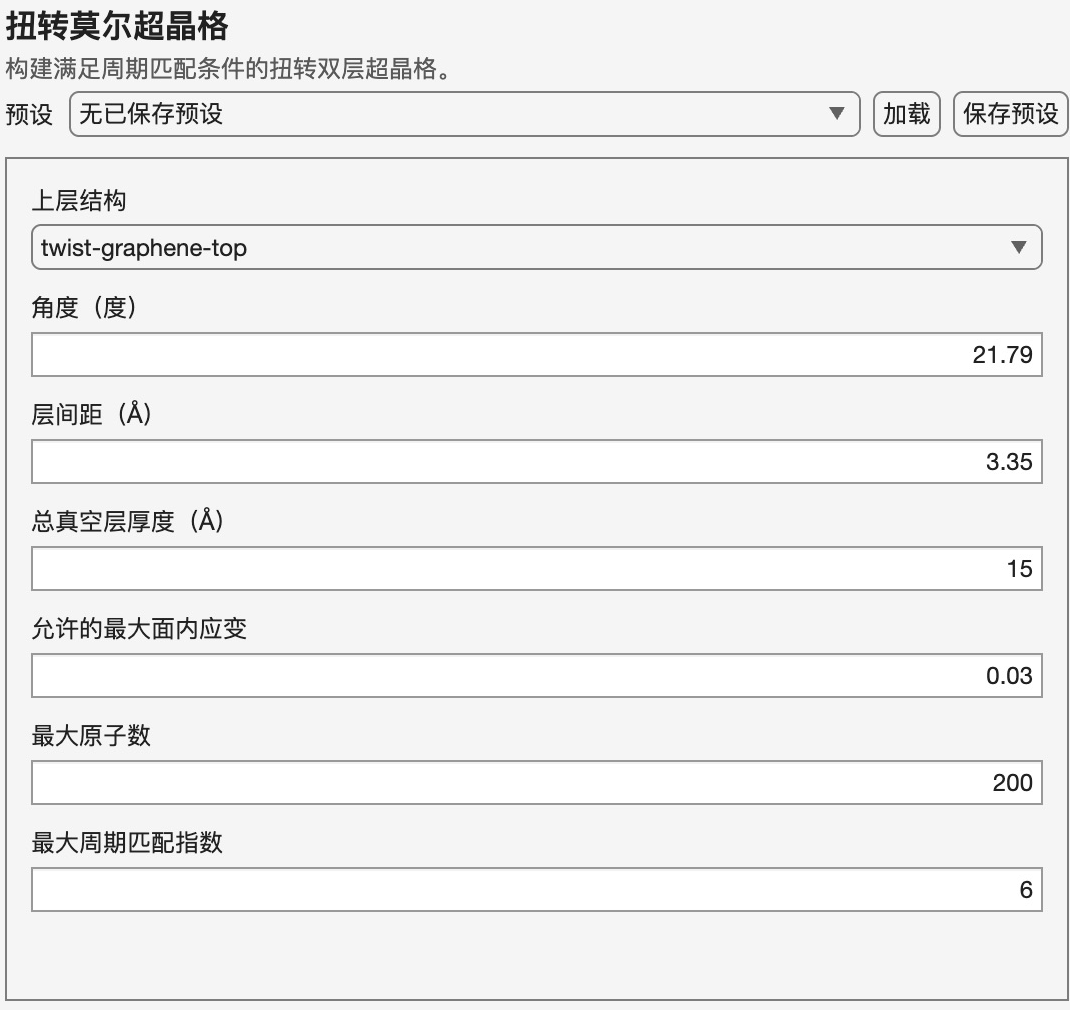
\includegraphics[width=107mm]{publication-assets/crop-7c221ceb9a35fdad53a3.png}
\par\vspace{2mm}

\includegraphics[width=60mm]{publication-assets/crop-faecdf5879e359505e34.png}
\caption{扭轉引數與預覽結果。目標角輸入21.786789度；數值框失去焦點後按顯示精度呈現為21.79。上層在圖中保留匯入時的名稱\file{twist-graphene-top}，對應本節的\file{twist-top}；預覽生成28個位點。}
\label{fig:online-twist-parameters}
\end{figure}

\begin{figure}[H]
\centering
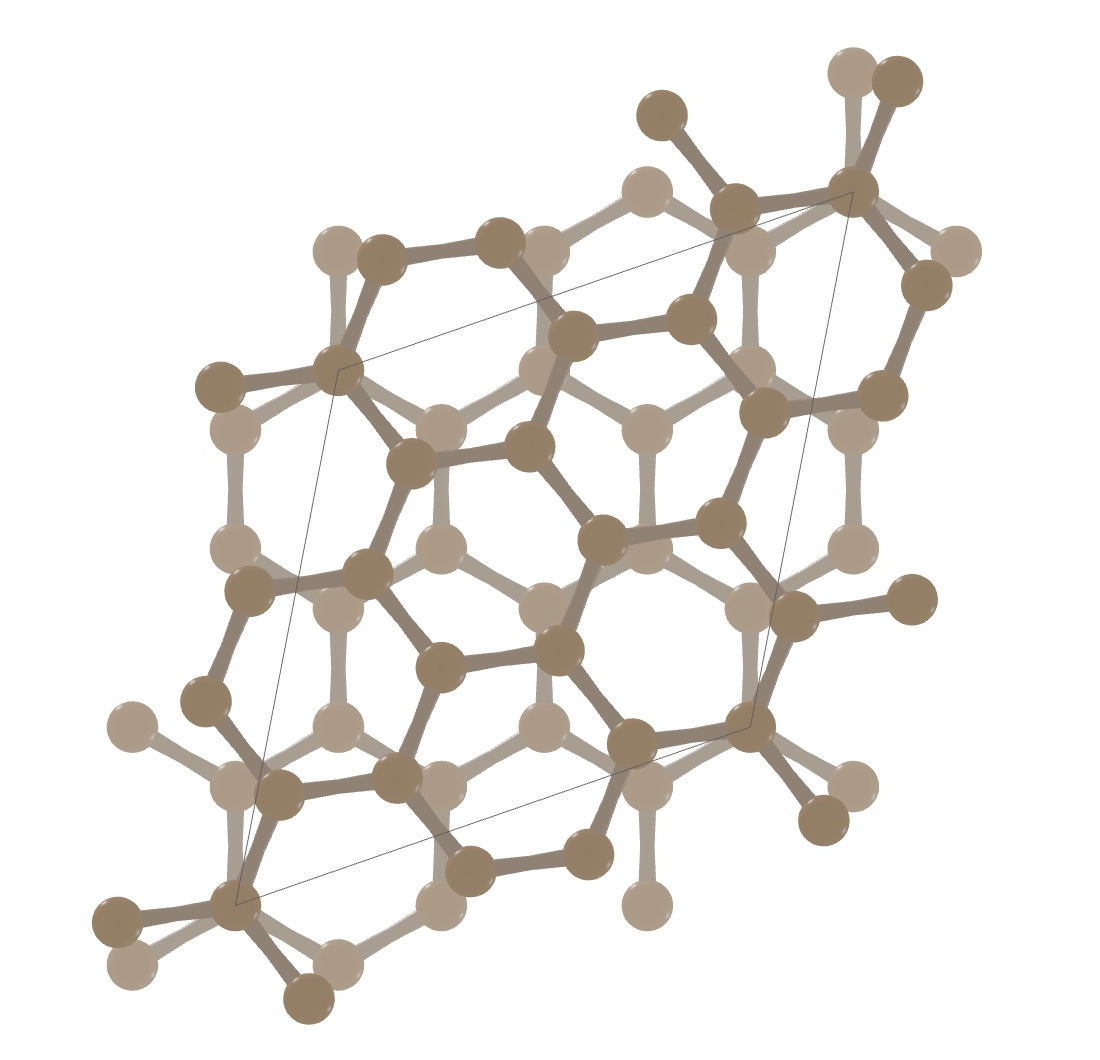
\includegraphics[width=93mm]{publication-assets/crop-89eb072a4598add87b05.png}
\caption{石墨烯扭轉雙層的法向檢視。兩層的六元環相對轉動；28個模型位點按當前週期範圍顯示為68個原子。}
\label{fig:online-twist-top}
\end{figure}

\subsection{讀懂生成的晶胞}

隨書\file{graphene-twist-21p786789.json}是按上述引數得到的參考結構，另提供幾何交換用的同名 CIF。模型有 28 個 C 位點，分為兩層，每層 14 個。與原始每層兩個位點相比，每一層的面內面積擴大為原來的 7 倍。

面內兩個晶格向量等長，均約為 $6.508548\,\text{\AA}$。相應面積約為 $36.6859\,\text{\AA}^2$。本例的新面內夾角為 $60^\circ$；輸入原胞的夾角為 $120^\circ$，兩者是不同的晶格基底表示，不能只憑角度改變就判斷晶體被拉歪。核對長度、面積、位點數與兩層的週期連線，應當放在一起進行。

對於這組石墨烯輸入，週期邊長也可用 $\sqrt{7}\times2.46\,\text{\AA}$ 核對，約為 $0.651\,\mathrm{nm}$。這裡的週期描述共同晶胞在面內的重複長度，不是層間距離，也不是某條 C--C 鍵長。模型中每層最短近鄰距離仍約為 $1.420282\,\text{\AA}$，與輸入單層一致。

從側面看，兩層相隔 $3.35\,\text{\AA}$，法向胞高為 $18.35\,\text{\AA}$。這組模型中每層原子各在一個平面內，所以本例胞高等於層間距與總真空之和。總真空 $15\,\text{\AA}$ 是整個薄片之外的空白高度；它不表示薄片上方和下方各有 $15\,\text{\AA}$。

\begin{figure}[H]
\centering
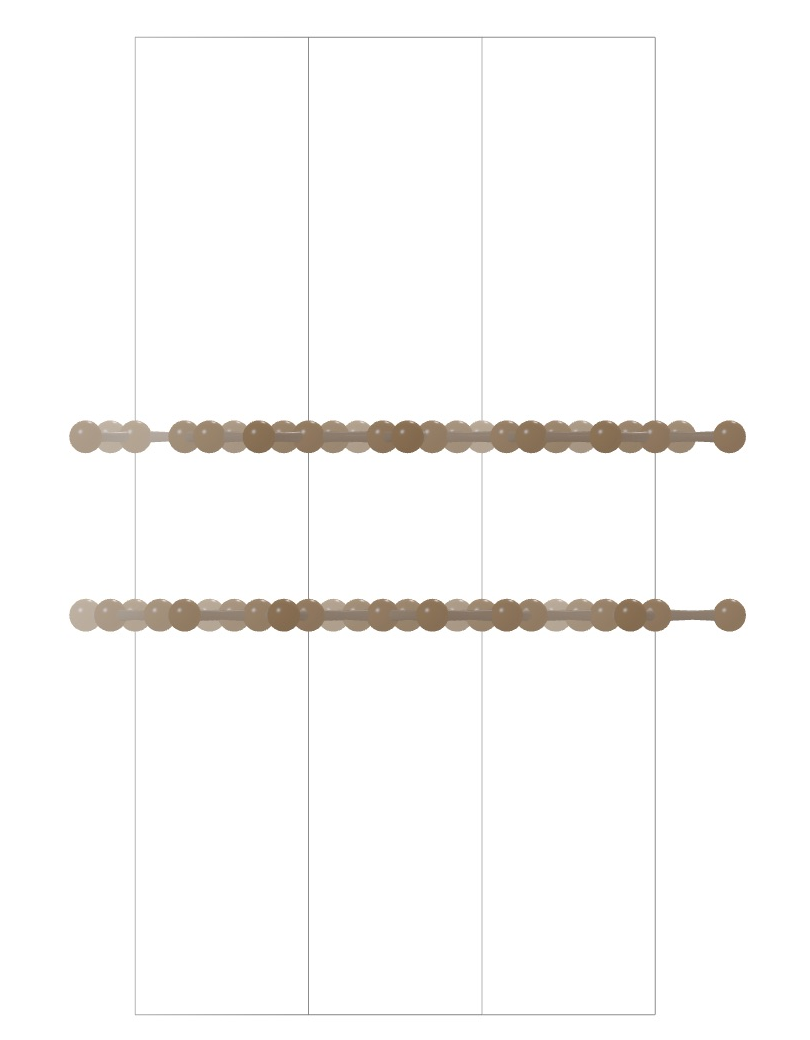
\includegraphics[width=67mm]{publication-assets/crop-a8d161a93e2745b16ef3.png}
\caption{同一模型的側視。兩張原子平面與法向晶胞邊界一起顯示，便於分辨層間距離和外側真空。}
\label{fig:online-twist-side}
\end{figure}

隨書參考結構的實際匹配角為 $21.786789298^\circ$，與目標角相差約 $2.98\times10^{-7}$ 度，面內應變為 0。檢查兩層近鄰鍵的方向，也可得到這一相對角度。

精確的角度和匹配資訊儲存在原生 JSON 的\file{properties}下的\file{moire}部分。用普通文字編輯器開啟本例 JSON，搜尋\file{achieved_angle_degrees}即可找到實際角；\file{target_angle_degrees}是目標角，\file{angle_error_degrees}是兩者的偏差，\file{in_plane_strain}是面內應變。對自己生成的結構，在檢視器的\ui{Export file}中選擇\ui{Structure file}，再選 JSON 匯出。不應選擇同一選單裡的\ui{Scene JSON}，後者儲存檢視場景，不能用來查詢上述結構匹配資訊。

\subsection{目標角與實際角為什麼可能不同}

目標角的輸入範圍為 $0^\circ$ 到 $60^\circ$。按六方面內晶格的對稱關係，工具把實際匹配角表示在 $0^\circ$ 到 $30^\circ$ 之間；比較較大目標角時，也應按這一表示約定檢視結果。本節先在這個較小範圍內練習，便於直接比較目標值與實際值。

共同週期只能由特定整數關係構成。輸入一個任意小數角，並不意味著一定存在大小合適、又完全等於該角的週期胞。本例把目標改成 $22^\circ$，保持其他引數不變，仍然得到 28 位點結構，實際角仍約為 $21.786789298^\circ$，角度偏差約為 $0.213211^\circ$。

這兩次構建具有相同的最終幾何，卻對應不同的目標輸入。隨書\file{graphene-twist-target22.json}保留了第二次結果，便於比較。報告模型時，應記錄實際角，而不是隻把引數視窗中輸入的目標角寫進圖題。

\begin{table}[htbp]
\centering
\caption{本組輸入下目標角與規模限制的實際對照。}
\begin{tabularx}{\linewidth}{lX}
\toprule
輸入變化 & 實際生成結果\\
\midrule
目標 $21.786789^\circ$，上限200 & 28位點，實際約 $21.786789298^\circ$。\\
目標 $22^\circ$，上限200 & 仍為28位點和同一實際角，偏差約 $0.213211^\circ$。\\
目標 $21.786789^\circ$，上限24 & 本例選擇4位點、接近 $0^\circ$ 的匹配，未達到原目標。\\
\bottomrule
\end{tabularx}
\end{table}

第三行說明，完成構建與達到目標角是兩項不同的檢查。28位點的匹配被上限24排除後，工具會在剩餘範圍內選擇結果。構建後，看到數量與預期明顯不同，應回到引數和實際角一起核對，再決定是否增大搜尋範圍。

較小轉角通常需要較長的共同週期和更多原子。比較不同轉角時，可以先固定層間距與應變要求，再逐步增加允許的模型規模和匹配指數。這樣更容易看清新增的搜尋範圍究竟改善了角度匹配，還是隻帶來更大的結構。本節約 $21.8^\circ$ 的例子使用較小整數，適合作為操作和週期檢查的起點。

\subsection{按研究目的選擇組裝入口}

\ui{介面建模}選單把幾種組裝方式放在一起。選擇時，先明確已經知道哪些幾何關係，再決定讓工具尋找什麼。

\begin{table}[htbp]
\centering
\caption{直接插入、層匹配與扭轉構建的選擇。}
\begin{tabularx}{\linewidth}{lX}
\toprule
入口 & 適合開始的情形\\
\midrule
插入結構 & 兩部分的位置已經確定，只需給出相對平移；保留當前宿主晶胞。\\
堆疊異質結構 & 希望比較共同面內晶胞，從允許應變、重複範圍與旋轉範圍中選擇候選。\\
扭轉莫爾超晶格 & 已有六方單層和目標轉角，希望尋找相應的整數共同週期。\\
\bottomrule
\end{tabularx}
\end{table}

在\ui{堆疊異質結構}的候選表中，面積、應變、原子數和旋轉角各自回答不同問題。面積與原子數反映計算規模；應變說明原始晶格需要改變多少才能匹配；旋轉角說明兩層如何相對定向。應變很小的候選也可能很大，面積最小的候選也可能需要較大形變。先比較這些量，再看具體原子排列，選擇會更有依據。

本節的扭轉命令則先利用六方整數關係確定一組共同週期，再組裝兩層。它不會要求在同一個視窗中填寫\ui{候選序號}。如果希望比較目標 $21.786789^\circ$ 與 $22^\circ$，應分別從兩張原始單層構建，分別記錄結果，而不是在前一個已完成的雙層上再次施加相同命令。

同樣，直接旋轉螢幕上的觀察方向只會改變視角；選擇一組原子進行旋轉則改變原子位置。兩者都不能代替共同晶胞的週期匹配。檢查扭轉模型時，除觀察兩層取向，還應顯示晶胞邊框，沿兩個面內方向檢視重複後的連線，確認區域性圖案與整個週期表達的是同一模型。

這組入口用於沿法向疊放的層狀介面。構建面內並排相接的異質結時，需另行準備結區的原子排列與邊界。

\subsection{進一步建立石墨烯/h-\headinglatin{BN}扭轉異質結構}

扭轉不只用於同一種材料的雙層。前面石墨烯與 h-BN 的零轉角匹配，主要展示兩種面內晶格常數如何協調；在此基礎上，還可以同時引入相對轉角。本例仍使用石墨烯作為底層，h-BN 作為上層：石墨烯晶格常數為 $2.46\,\text{\AA}$，h-BN 為 $2.50\,\text{\AA}$。

\begin{steps}
  \item 重新匯入\file{twist-graphene-bottom.json}與\file{hBN-layer.json}，分別命名為\file{graphene-bottom}和\file{hBN-top}。不要把前一個已經扭轉的雙層作為底層。
  \item 啟用新的石墨烯單層，在\ui{扭轉莫爾超晶格}中將\ui{上層結構}選擇為\file{hBN-top}。
  \item 沿用表中的目標角、層間距、總真空、200位點上限與匹配指數6，允許最大面內應變仍設為0.03。
  \item 預覽後核對組成應為 $\mathrm{C_{14}B_7N_7}$，共28個位點。上層和底層各有14個位點，但元素組成不同。
  \item 應用並儲存為\file{graphene-hBN-twist-21p786789}，再與零轉角的\file{graphene-hBN-stacked.json}比較。
\end{steps}

本例實際角同樣約為 $21.786789298^\circ$，面內主應變為 0.016，即 1.6\%。h-BN 的面內尺寸被匹配到石墨烯共同晶格，層間距仍為 $3.35\,\text{\AA}$，法向胞高仍為 $18.35\,\text{\AA}$。應變和轉角描述的是不同變化：前者調整尺寸，後者改變兩層的相對方向。

兩種構建命令得到的都是幾何模型。研究介面電荷轉移、能帶對齊或結區性質時，需要在儲存的結構上繼續建立相應計算，並區分構建輸入的層間距與計算後得到的距離。

\subsection{儲存扭轉模型}

儲存專案可以保留輸入層、生成結構和後續工作流。單獨交換結構時，本組提供 JSON 與 CIF 兩種格式：JSON保留面內/法向週期標記、層編號和扭轉匹配資訊；CIF便於交換晶胞與原子位置。匯入本組CIF時，三個方向均按週期處理，莫爾匹配資訊需另行保留。繼續本章的二維建模比較，優先使用JSON；使用CIF進入其他計算流程時，再按目標方法確認法向邊界與真空設定。

\begin{steps}
  \item 為每個結果寫清材料、實際角和主要變化，例如“石墨烯雙層，實際21.7868度”，不要只儲存\file{result}之類的通用名稱。
  \item 記錄輸入層的晶格、目標角與實際角、應變、層間距、總真空、位點數及面內週期。比較表可將這些量各佔一列。
  \item 儲存專案後重新開啟，再檢查上下兩層的組成和晶胞。匯出結構時，保留對應的引數記錄，便於解釋另一個軟體中看到的模型。
  \item 需要重複生成時，以\file{-nojvm}啟動MATLAB\regmark{}，配置好工具箱路徑後，從隨書示例目錄執行\file{twist_examples.m}；只檢查已儲存檔案時，執行\file{verify_twist_examples.m}。
\end{steps}

隨書結構是用於後續弛豫和電子結構計算的初始模型。比較扭角效應時，採用一致的泛函、贗勢、截斷能和合適的取樣條件，並將計算設定與結構一同儲存。
